Figures \ref{fig:inj_125_7-8TeV}-\ref{fig:inj_200} summarize the results for various 8 TeV analysis 
configurations in the presence of SM Higgs with \mHi=125 \GeV\ and \mHi=200 \GeV\ respectively.
For each analysis, toy experiments are made based on poisson sampling on the expected yield 
and shapes where background estimates are not re-evaluated for each toy.
For the moment only 100 toy experiment per analysis are simulated due to the long computational time required; 
this limitation causes a few fluctuations in the results, but the overall trend is clear.

\begin{figure}[!hbtp]
\centering
\subfigure[limit]{
\centering
\label{subfig:limit_allcomb_inj125}
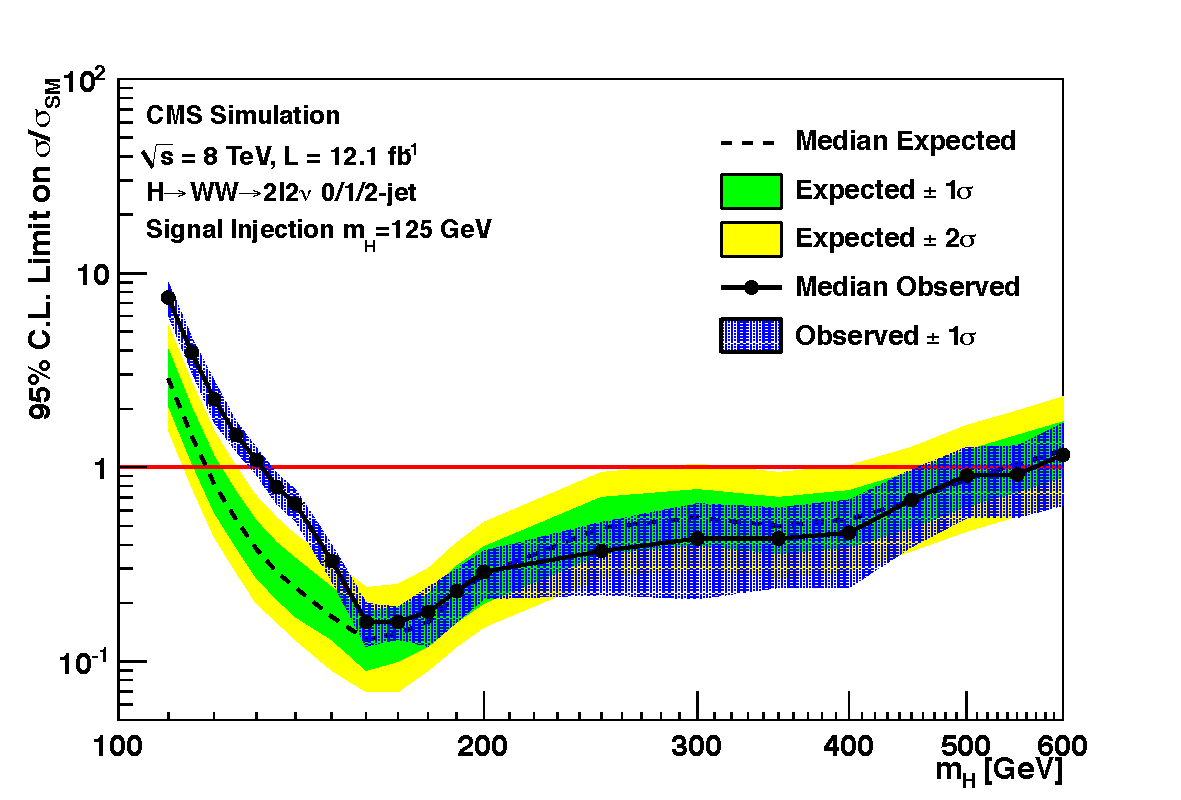
\includegraphics[width=.45\textwidth]{figures/limit_allcomb_inj125.pdf}
}
\subfigure[significance]{
\centering
\label{subfig:signif_allcomb_inj125}
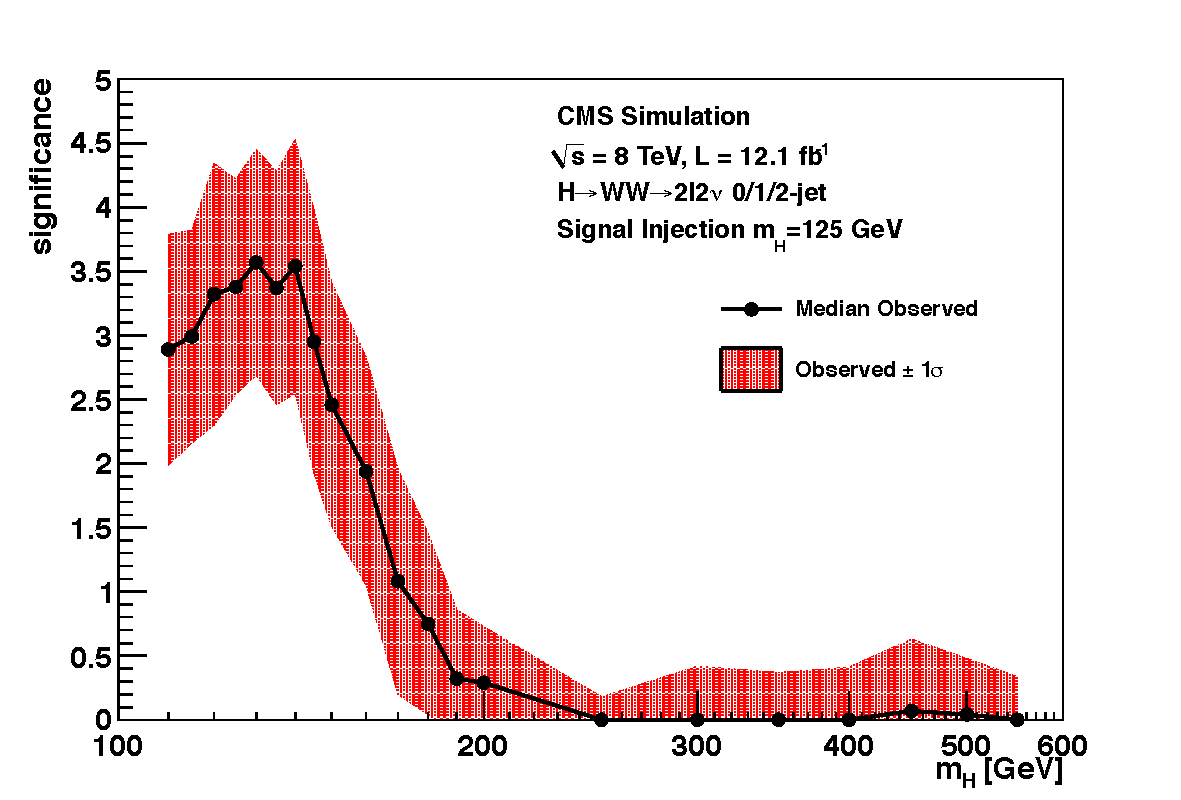
\includegraphics[width=.45\textwidth]{figures/signif_allcomb_inj125.pdf}
}
\caption{Limits and significance in presence of SM Higgs with \mHi=125 \GeV for the default analysis combining 7 TeV and 8 TeV data.}
\label{fig:inj_125_7-8TeV}
\end{figure}

\begin{figure}[!hbtp]
\centering
\subfigure[limit (cut 0/1/2-j, OF+SF)]{
\centering
\label{subfig:limit_cut_inj125}
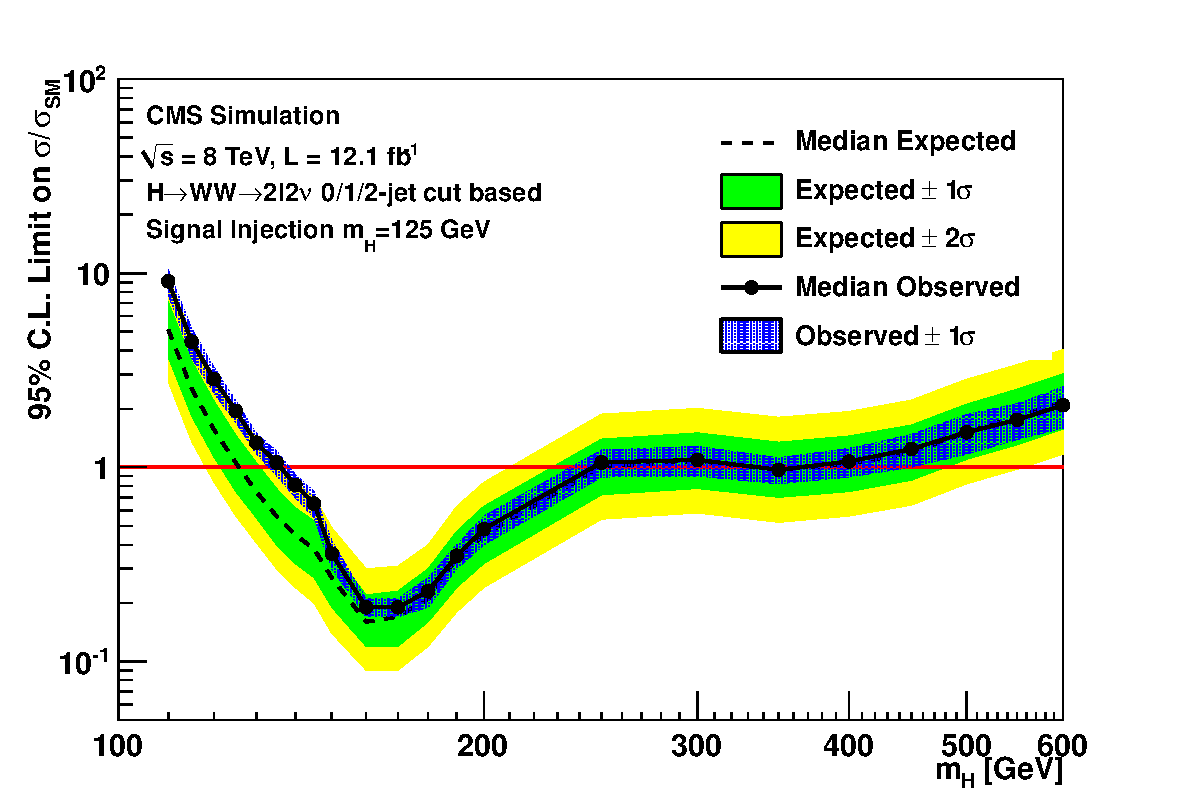
\includegraphics[width=.45\textwidth]{figures/limit_cut_inj125.pdf}
}
\subfigure[significance (cut 0/1/2-j, OF+SF)]{
\centering
\label{subfig:signif_cut_inj125}
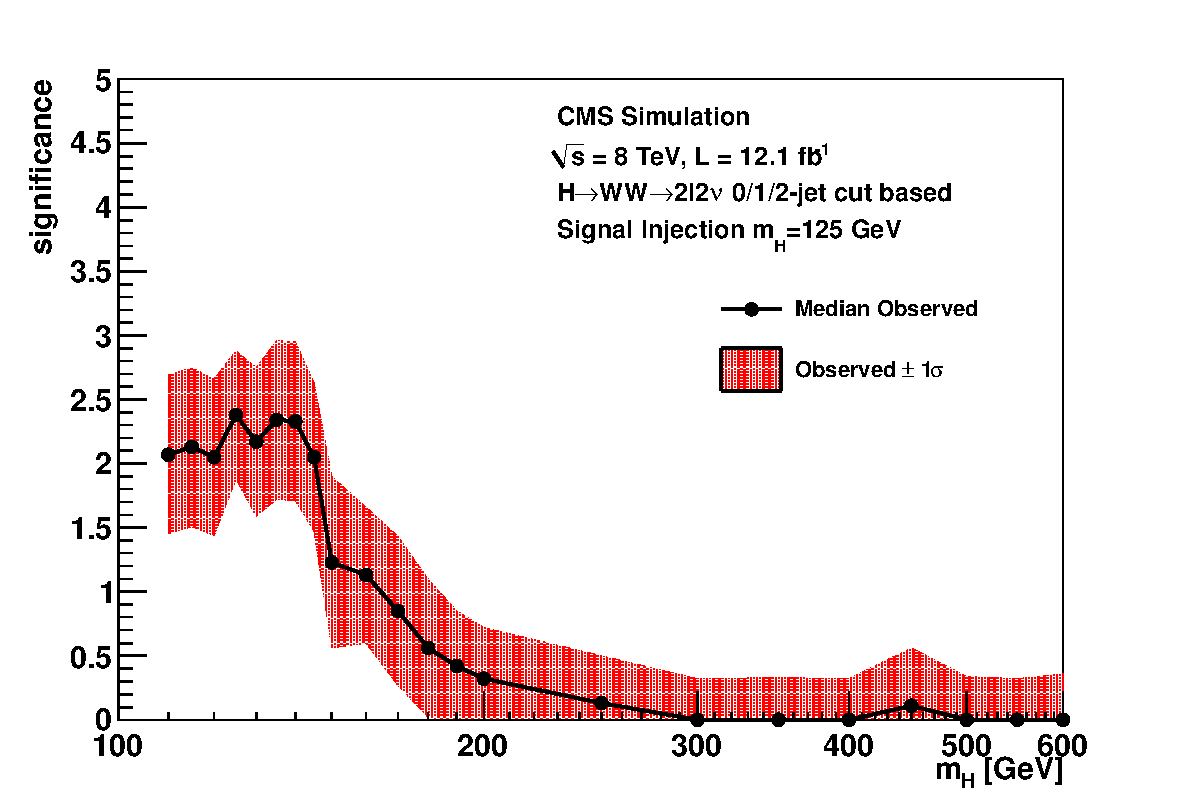
\includegraphics[width=.45\textwidth]{figures/signif_cut_inj125.pdf}
}
\\
\subfigure[limit (2D 0/1-j OF)]{
\centering
\label{subfig:limit_shape_inj125}
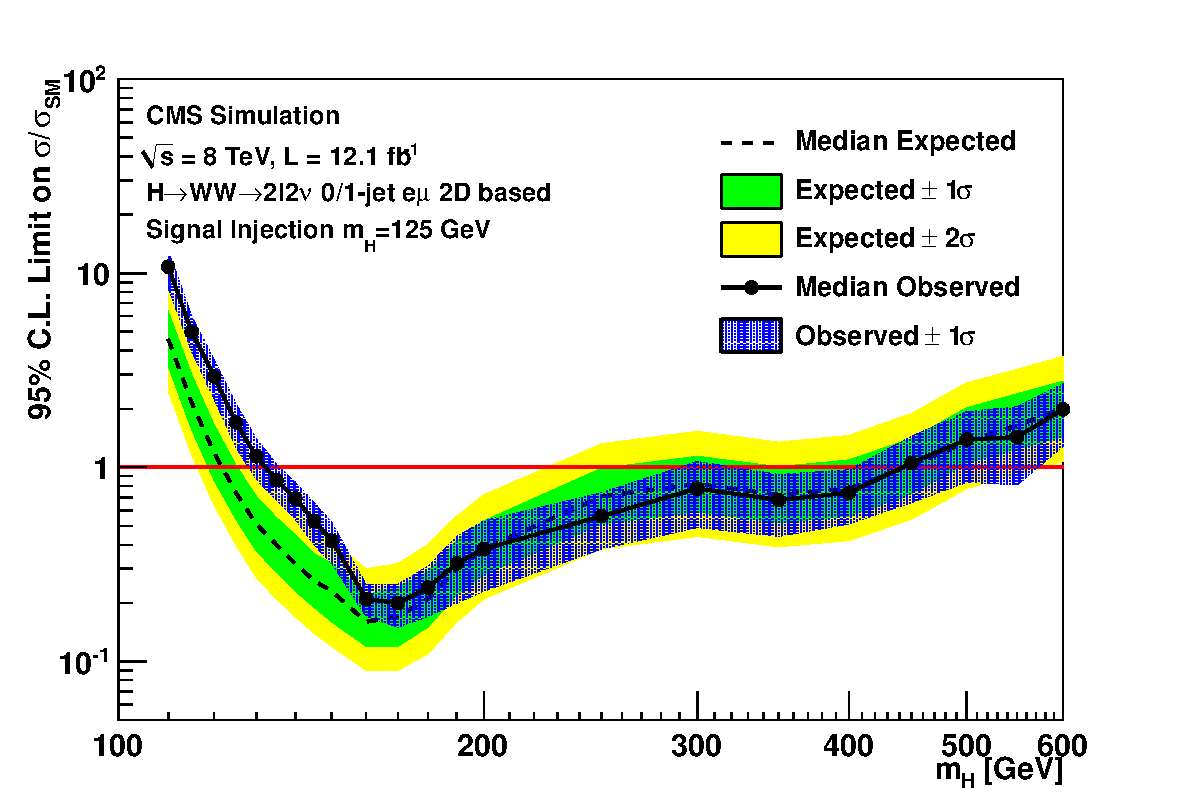
\includegraphics[width=.45\textwidth]{figures/limit_shape_inj125.pdf}
}
\subfigure[significance (2D 0/1-j OF)]{
\centering
\label{subfig:signif_shape_inj125}
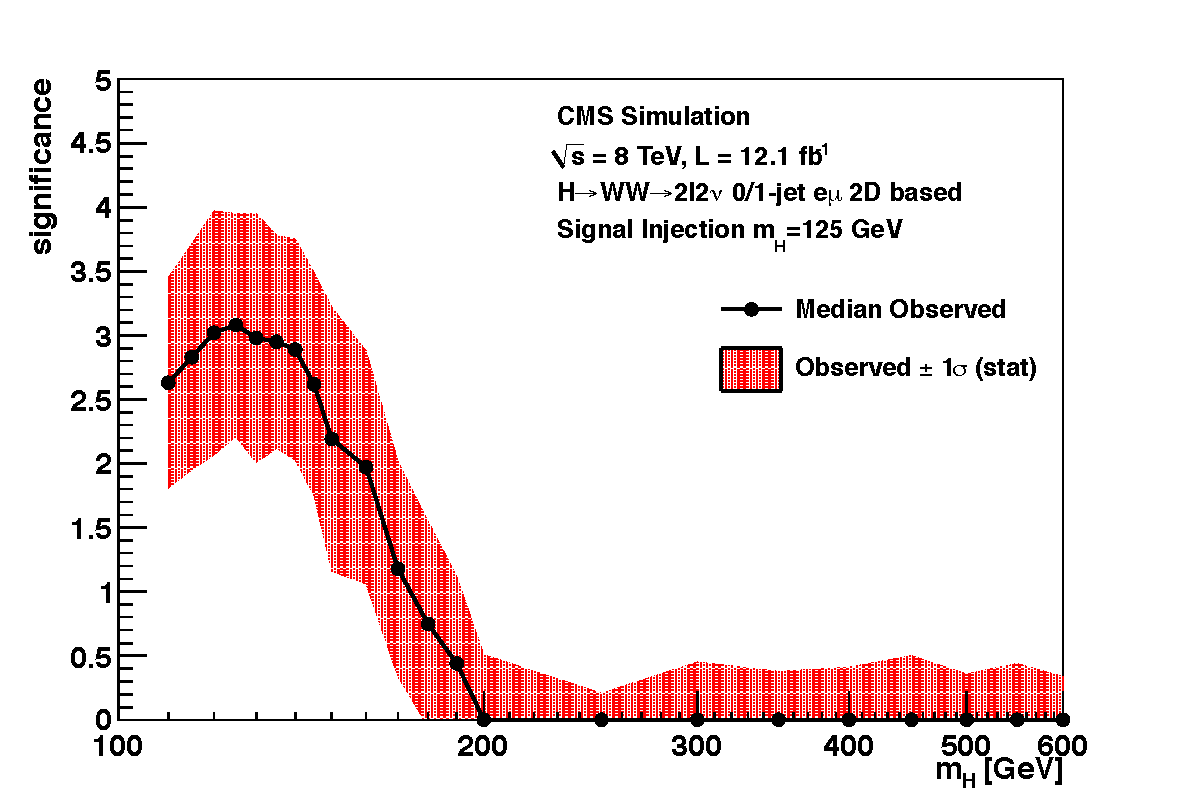
\includegraphics[width=.45\textwidth]{figures/signif_shape_inj125.pdf}
}
\\
\subfigure[limit 2D+cut]{
\centering
\label{subfig:limit_combine_inj125}
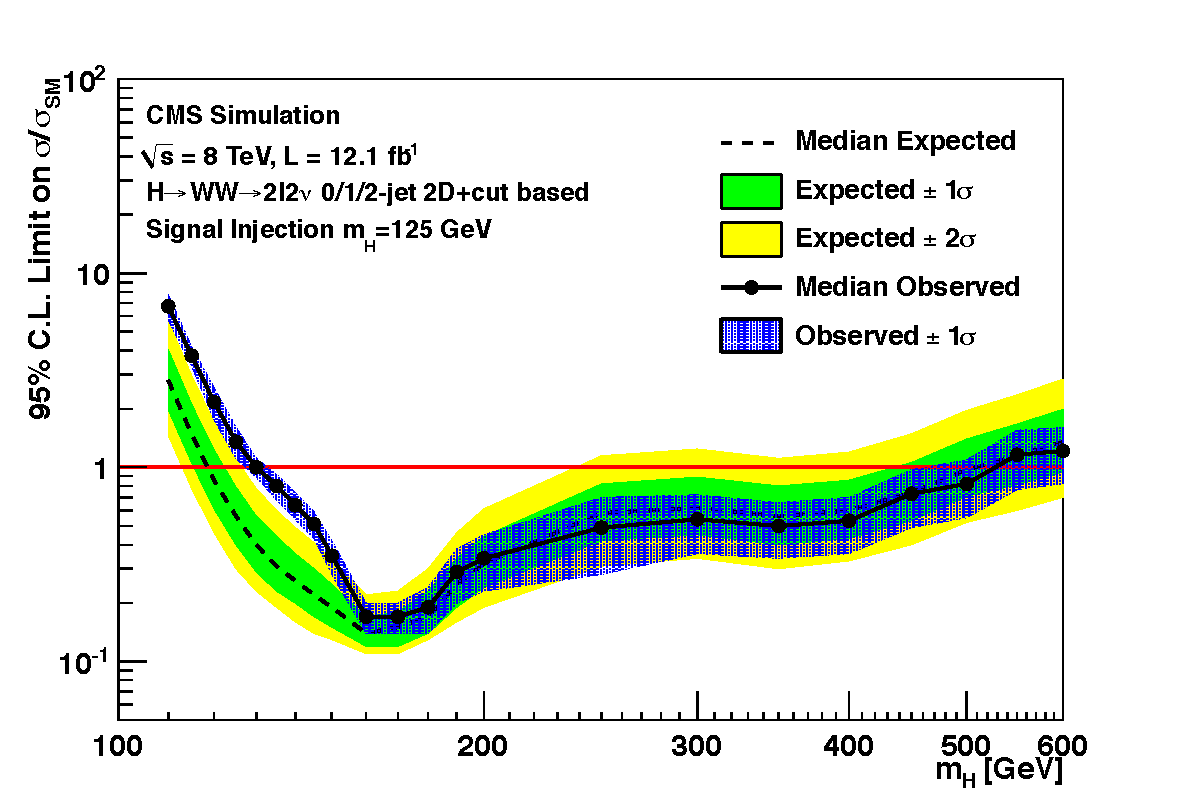
\includegraphics[width=.45\textwidth]{figures/limit_combine_inj125.pdf}
}
\subfigure[significance 2D+cut]{
\centering
\label{subfig:signif_combine_inj125}
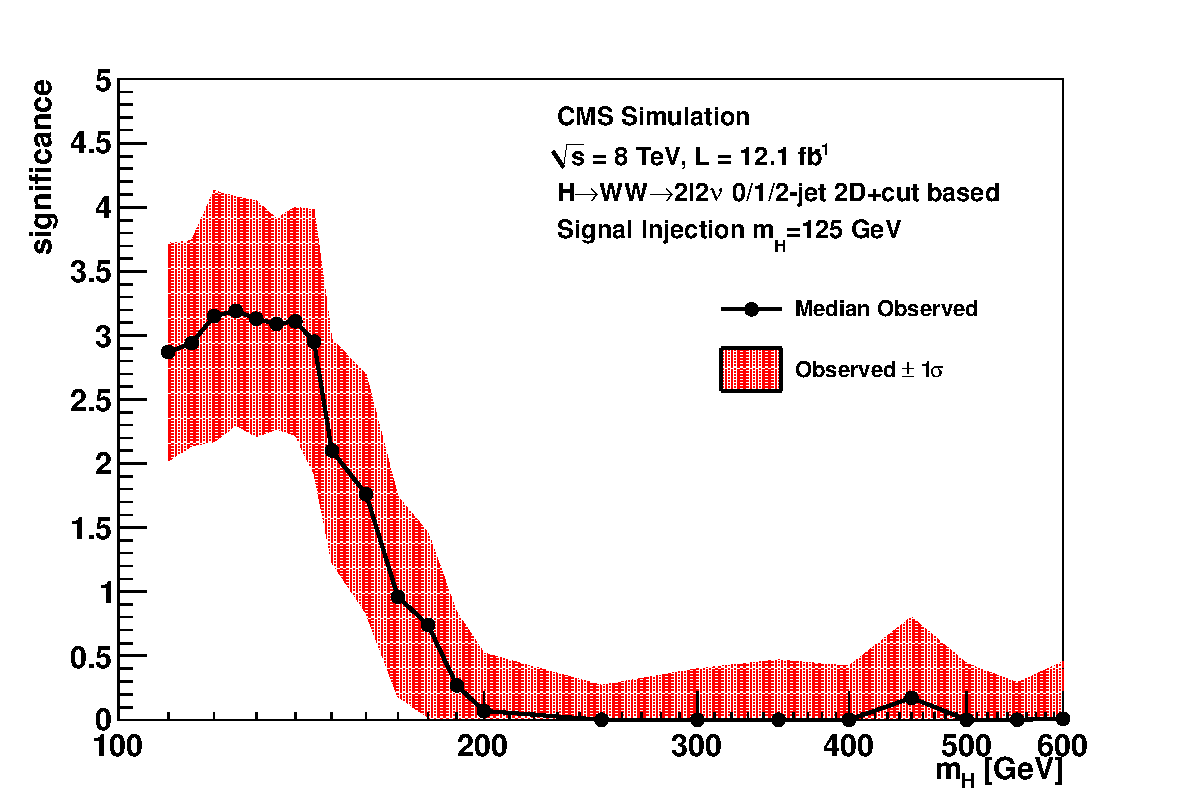
\includegraphics[width=.45\textwidth]{figures/signif_combine_inj125.pdf}
}
\caption{Limits and significance in presence of SM Higgs with \mHi=125 \GeV (8 TeV only).}
\label{fig:inj_125}
\end{figure}


\begin{figure}[!hbtp]
\centering
\subfigure[limit (cut 0/1/2-j, OF+SF)]{
\centering
\label{subfig:limit_cut_inj200}
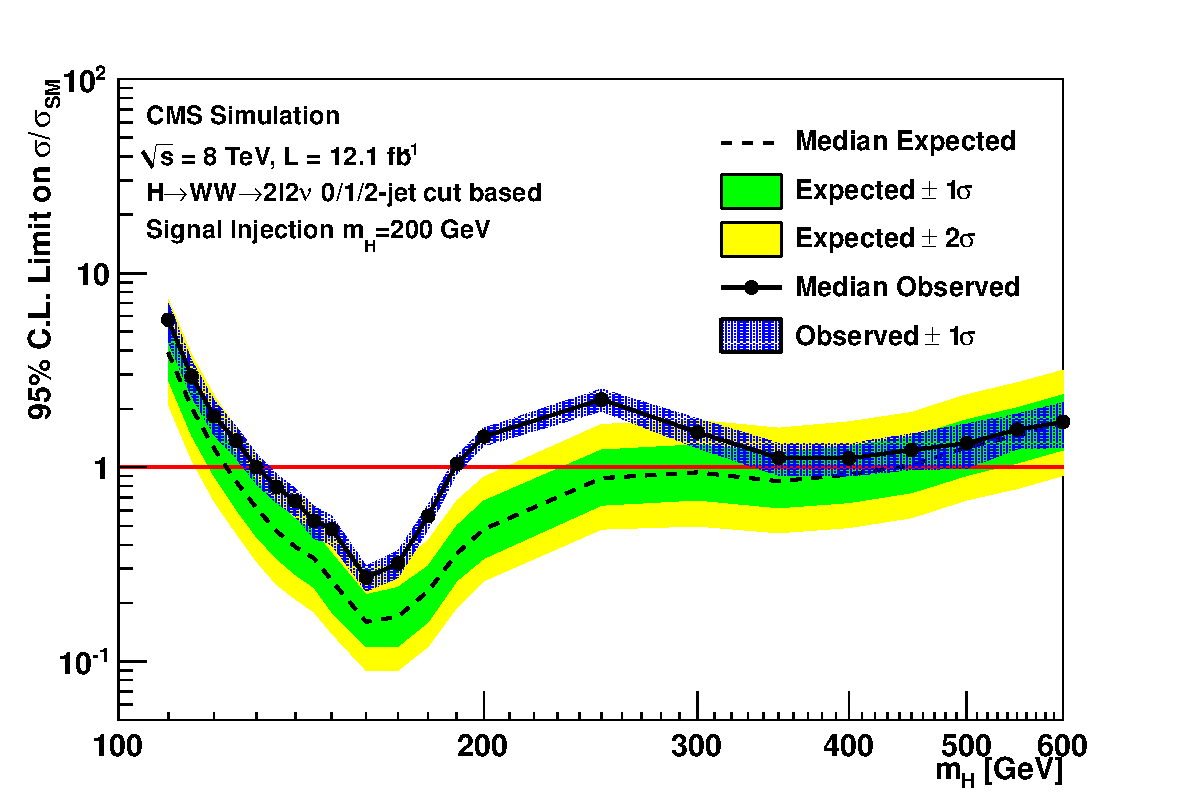
\includegraphics[width=.45\textwidth]{figures/limit_cut_inj200.pdf}
}
\subfigure[significance (cut 0/1/2-j, OF+SF)]{
\centering
\label{subfig:signif_cut_inj200}
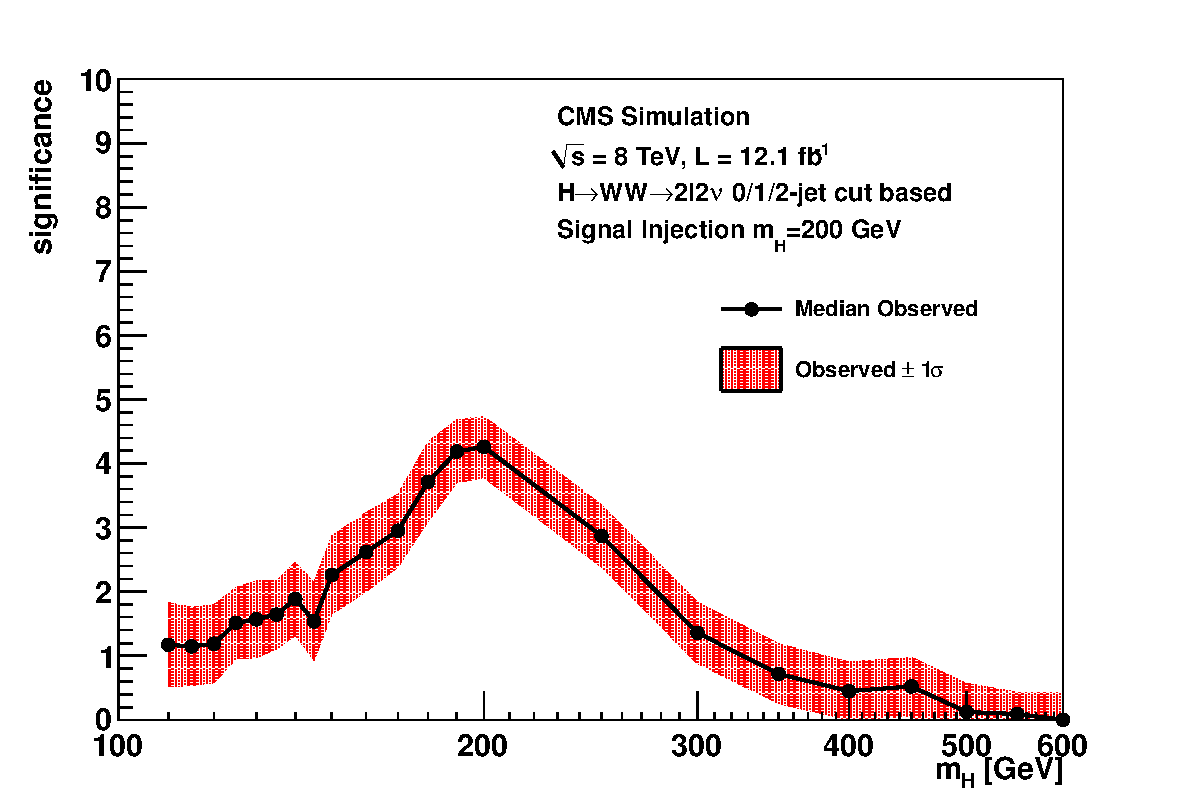
\includegraphics[width=.45\textwidth]{figures/signif_cut_inj200.pdf}
}
\\
\subfigure[limit (2D 0/1-j OF)]{
\centering
\label{subfig:limit_shape_inj200}
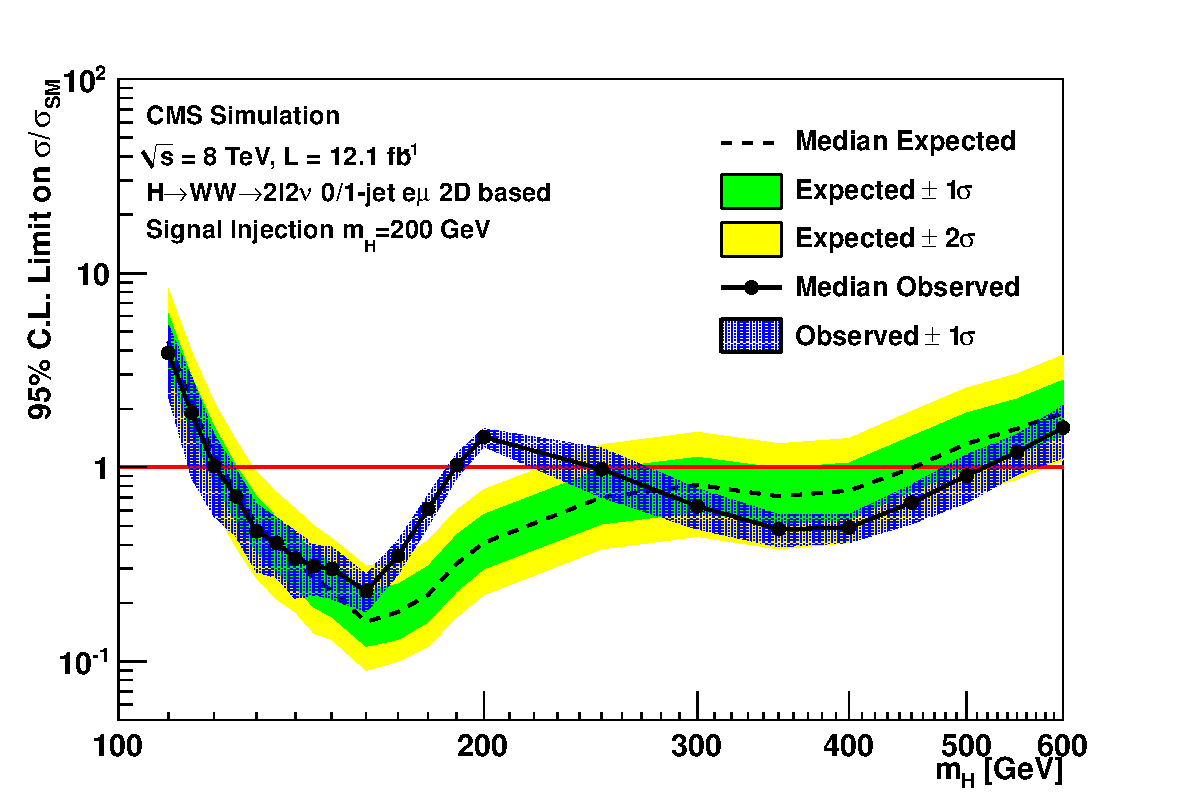
\includegraphics[width=.45\textwidth]{figures/limit_shape_inj200.pdf}
}
\subfigure[significance (2D 0/1-j OF)]{
\centering
\label{subfig:signif_shape_inj200}
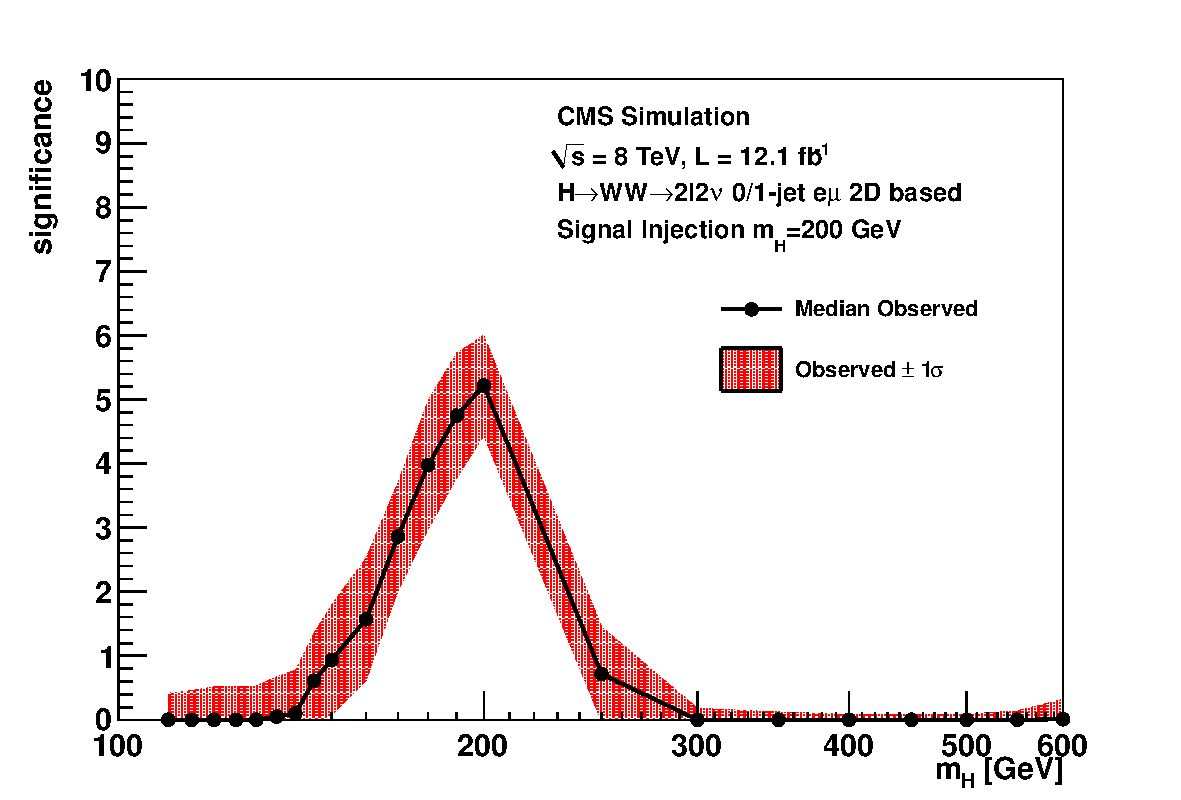
\includegraphics[width=.45\textwidth]{figures/signif_shape_inj200.pdf}
}
\\
\subfigure[limit 2D+cut]{
\centering
\label{subfig:limit_combine_inj200}
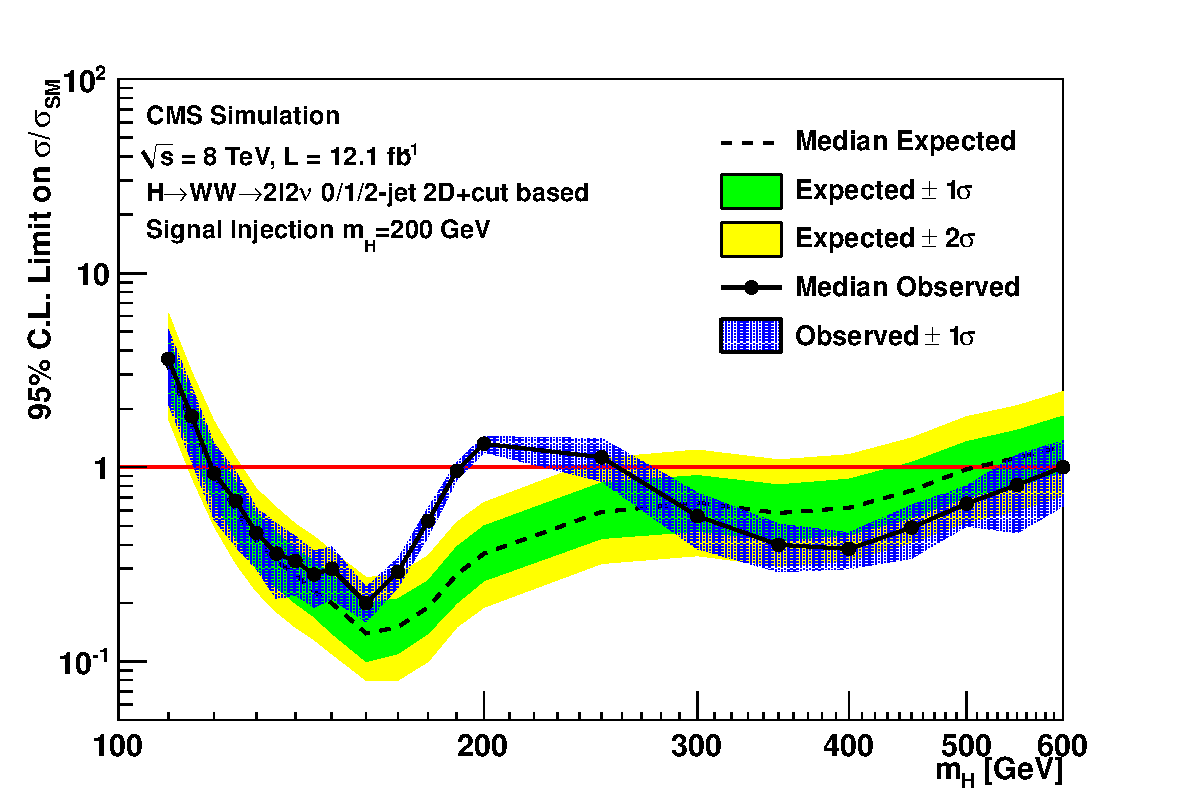
\includegraphics[width=.45\textwidth]{figures/limit_combine_inj200.pdf}
}
\subfigure[significance 2D+cut]{
\centering
\label{subfig:signif_combine_inj200}
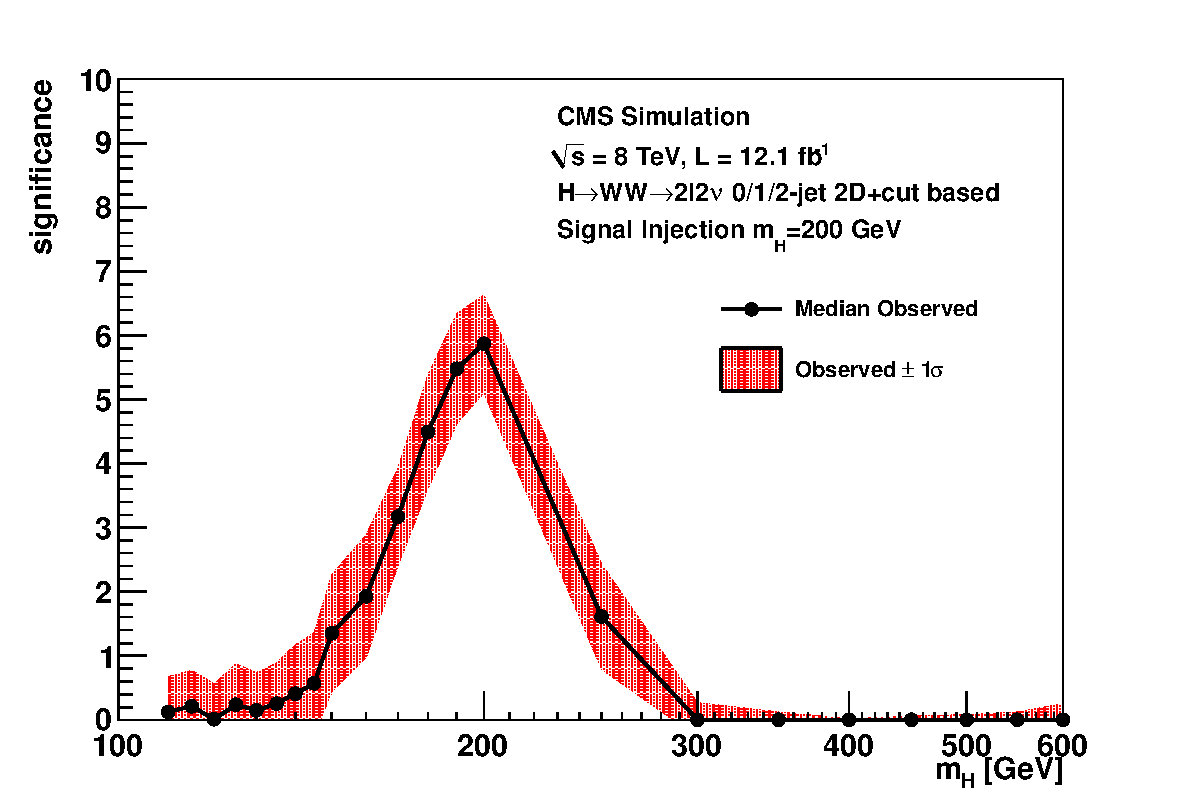
\includegraphics[width=.45\textwidth]{figures/signif_combine_inj200.pdf}
}
\caption{Limits and significance in presence of SM Higgs with \mHi=200 \GeV (8 TeV only).}
\label{fig:inj_200}
\end{figure}

\clearpage
